% blog-title: Exponential Families for Bandit Models
% blog-date: 2026-06-20
% blog-description: A polished note on exponential families as one likelihood language for estimation, concentration, KL-UCB, and Thompson sampling.
% blog-lang: en

\documentclass[en,nofont,11pt]{elegantbook}

\title{Exponential Families for Bandit Models}
\subtitle{The Natural Language of Modern Bandit Models}
\author{Tang}
\institute{Tang's Machine Learning Blog}
\date{2026-06-20}
\version{1.0.0}
\bioinfo{Topic}{Exponential Families, KL-UCB, Thompson Sampling}
\cover{assets/blog-cover.jpg}

\usepackage{fontspec}
\ifdefined\setCJKmainfont
\else
  \usepackage[UTF8,scheme=plain,fontset=none]{ctex}
\fi
\usepackage{xcolor}
\usepackage{listings}
\usepackage{float}
\usepackage{tcolorbox}
\tcbuselibrary{breakable, listings, skins}
\usetikzlibrary{arrows.meta,positioning,calc,decorations.pathmorphing,decorations.pathreplacing,fit,backgrounds,patterns,shapes.geometric}

\IfFontExistsTF{Microsoft YaHei}{
  \setCJKmainfont{Microsoft YaHei}
  \setCJKsansfont{Microsoft YaHei}
  \setCJKmonofont{Microsoft YaHei UI}
}{
  \IfFontExistsTF{Noto Serif CJK SC}{
    \setCJKmainfont{Noto Serif CJK SC}
    \setCJKsansfont{Noto Sans CJK SC}
    \setCJKmonofont{Noto Sans Mono CJK SC}
  }{}
}

\definecolor{blogAccent}{HTML}{1F6F8B}
\definecolor{blogInk}{HTML}{172026}
\definecolor{blogCodeBg}{HTML}{F5F7F8}
\definecolor{blogCodeBorder}{HTML}{D6E2E8}
\definecolor{blogKeyword}{HTML}{B23A48}
\definecolor{blogString}{HTML}{287D4F}
\definecolor{blogComment}{HTML}{687783}

\lstdefinestyle{blogcode}{
  basicstyle=\ttfamily\small,
  keywordstyle=\bfseries\color{blogKeyword},
  stringstyle=\color{blogString},
  commentstyle=\itshape\color{blogComment},
  numberstyle=\scriptsize\color{blogComment},
  numbers=left,
  numbersep=8pt,
  showstringspaces=false,
  breaklines=true,
  tabsize=2,
  columns=fullflexible,
  keepspaces=true
}

\newtcblisting{codeblock}[2][]{
  listing only,
  breakable,
  enhanced,
  colback=blogCodeBg,
  colframe=blogCodeBorder,
  arc=2mm,
  boxrule=0.4pt,
  left=6mm,
  right=2mm,
  top=1mm,
  bottom=1mm,
  listing options={style=blogcode, language=#2},
  #1
}

\hypersetup{
  colorlinks=true,
  linkcolor=blogAccent,
  urlcolor=blogAccent,
  citecolor=blogAccent
}

\addbibresource{tex/bandits-references.bib}
\newcolumntype{L}[1]{>{\raggedright\arraybackslash}p{#1}}

\definecolor{expBlue}{RGB}{28,73,135}
\definecolor{expLightBlue}{RGB}{232,241,252}
\definecolor{expOrange}{RGB}{150,75,25}
\definecolor{expLightOrange}{RGB}{255,247,236}
\definecolor{expGreen}{RGB}{38,105,65}
\definecolor{expLightGreen}{RGB}{235,247,239}
\definecolor{expPurple}{RGB}{92,61,140}
\definecolor{expLightPurple}{RGB}{244,239,250}
\definecolor{expGray}{RGB}{247,247,247}
\colorlet{mainblue}{expBlue}
\colorlet{lightblue}{expLightBlue}
\colorlet{deeporange}{expOrange}
\colorlet{lightorange}{expLightOrange}
\colorlet{deepgreen}{expGreen}
\colorlet{softgreen}{expLightGreen}
\colorlet{deeppurple}{expPurple}
\colorlet{softpurple}{expLightPurple}
\colorlet{lightgray}{expGray}

\newtcolorbox{keyidea}[1][]{enhanced,breakable,colback=lightblue,colframe=mainblue,
  coltitle=white,fonttitle=\bfseries,title=Key idea,#1}
\newtcolorbox{thinkbox}[1][]{enhanced,breakable,colback=lightorange,colframe=deeporange,
  coltitle=white,fonttitle=\bfseries,title=Think,#1}
\newtcolorbox{resultbox}[1][]{enhanced,breakable,colback=white,colframe=mainblue,
  coltitle=white,fonttitle=\bfseries,title=Result,#1}
\newtcolorbox{patternbox}[1][]{enhanced,breakable,colback=softgreen,colframe=deepgreen,
  coltitle=white,fonttitle=\bfseries,title=Proof pattern,#1}
\newtcolorbox{researchbox}[1][]{enhanced,breakable,colback=softpurple,colframe=deeppurple,
  coltitle=white,fonttitle=\bfseries,title=Research lens,#1}

\newcommand{\E}{\mathbb{E}}
\newcommand{\Pbb}{\mathbb{P}}
\newcommand{\R}{\mathbb{R}}
\newcommand{\one}{\mathbf{1}}
\newcommand{\KL}{\operatorname{KL}}
\newcommand{\kl}{\operatorname{kl}}
\newcommand{\Ber}{\operatorname{Bern}}
\newcommand{\Poi}{\operatorname{Poisson}}
\newcommand{\Normal}{\mathcal{N}}
\newcommand{\Var}{\operatorname{Var}}
\newcommand{\Cov}{\operatorname{Cov}}
\newcommand{\argmax}{\operatorname*{arg\,max}}
\newcommand{\argmin}{\operatorname*{arg\,min}}
\newcommand{\dd}{\mathrm{d}}
\newcommand{\ind}{\mathbf{1}}

\begin{document}
\maketitle
\frontmatter
\tableofcontents
\mainmatter

\chapter{Three Reward Models, One Repeated Calculation}

A bandit can return very different kinds of rewards.

A recommendation is clicked or ignored. A sensor reports a real number with measurement noise. A server receives a count of requests during the next second. The first observation is binary, the second is continuous, and the third is a nonnegative integer.

At first these look like three unrelated statistical problems. Yet after a few observations, the learner keeps asking the same questions:

\begin{itemize}
\item What single number summarizes what this arm has shown so far?
\item Which parameter value makes those observations most plausible?
\item How quickly can a wrong parameter value be ruled out?
\item How should a prior belief be updated after one more reward?
\end{itemize}

For Bernoulli, Gaussian, and Poisson rewards, the algebra behind all four questions has the same shape. That shared shape is the exponential family.

The name can make the subject sound more exotic than it is. The central idea is modest:

\begin{center}
\emph{Put the unknown parameter next to a summary of the data, and place everything needed for normalization in one convex function.}
\end{center}

We will first see the pattern inside familiar distributions. Only then will we give it a name.

\section{Binary rewards: the data become a count}

Let $X\in\{0,1\}$ and let $p$ be the probability of a success. Then
\[
\Pbb_p(X=x)=p^x(1-p)^{1-x}.
\]
For observations $x_1,\ldots,x_n$,
\begin{align*}
L(p;x_1,\ldots,x_n)
&=\prod_{i=1}^{n}p^{x_i}(1-p)^{1-x_i}\\
&=p^{\sum_{i=1}^{n}x_i}(1-p)^{n-\sum_{i=1}^{n}x_i}.
\end{align*}
Define
\[
S_n=\sum_{i=1}^{n}x_i.
\]
Then
\[
L(p;x_1,\ldots,x_n)=p^{S_n}(1-p)^{n-S_n}.
\]
The order of clicks and non-clicks has disappeared. The likelihood remembers only how many clicks occurred.

\section{Gaussian rewards: the data become a sum}

Suppose $X\sim\Normal(\mu,\sigma^2)$ and the variance $\sigma^2$ is known. Its density is
\[
p_\mu(x)
=
\frac{1}{\sqrt{2\pi\sigma^2}}
\exp\left\{-\frac{(x-\mu)^2}{2\sigma^2}\right\}.
\]
For $n$ independent observations,
\begin{align*}
\log L(\mu)
&=
-\frac{n}{2}\log(2\pi\sigma^2)
-\frac{1}{2\sigma^2}\sum_{i=1}^{n}(x_i-\mu)^2\\
&=
-\frac{n}{2}\log(2\pi\sigma^2)
-\frac{1}{2\sigma^2}\sum_{i=1}^{n}x_i^2
+\frac{\mu}{\sigma^2}\sum_{i=1}^{n}x_i
-\frac{n\mu^2}{2\sigma^2}.
\end{align*}
As a function of $\mu$, the sample enters through
\[
S_n=\sum_{i=1}^{n}x_i.
\]
Again, the full history can be compressed to a running total.

\section{Count rewards: the data become a sum again}

Suppose $X\sim\Poi(\lambda)$. Then
\[
\Pbb_\lambda(X=x)
=
\frac{e^{-\lambda}\lambda^x}{x!},
\qquad x=0,1,2,\ldots.
\]
For $n$ independent observations,
\begin{align*}
L(\lambda)
&=\prod_{i=1}^{n}\frac{e^{-\lambda}\lambda^{x_i}}{x_i!}\\
&=\frac{1}{\prod_{i=1}^{n}x_i!}
\exp\left\{-n\lambda+\left(\sum_{i=1}^{n}x_i\right)\log\lambda\right\}.
\end{align*}
The parameter-dependent part again uses only
\[
S_n=\sum_{i=1}^{n}x_i.
\]

\begin{keyidea}
The exponential-family idea is already visible. A potentially long dataset is replaced by a short running summary. The model then compares that summary with what each parameter value predicts.
\end{keyidea}

\begin{figure}[H]
\centering
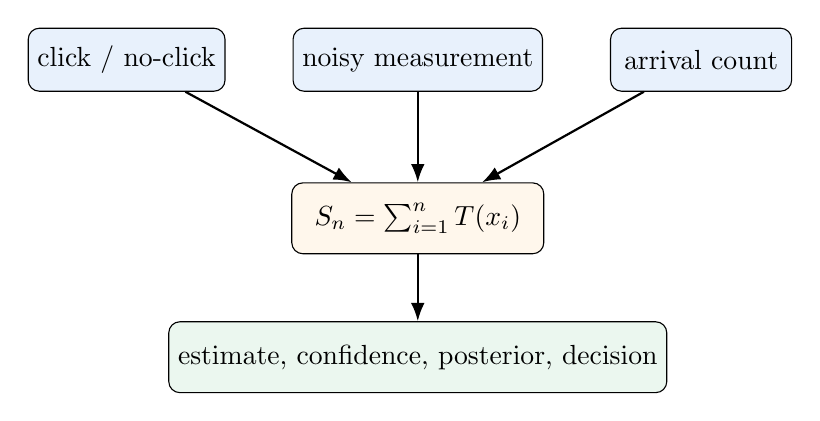
\begin{tikzpicture}[>=Latex,node distance=0.85cm]
\node[draw,rounded corners,fill=lightblue,minimum width=2.3cm,minimum height=0.8cm] (b) {click / no-click};
\node[draw,rounded corners,fill=lightblue,minimum width=2.3cm,minimum height=0.8cm,right=of b] (g) {noisy measurement};
\node[draw,rounded corners,fill=lightblue,minimum width=2.3cm,minimum height=0.8cm,right=of g] (p) {arrival count};
\node[draw,rounded corners,fill=lightorange,minimum width=3.2cm,minimum height=0.9cm,below=1.15cm of g] (s) {$S_n=\sum_{i=1}^{n}T(x_i)$};
\node[draw,rounded corners,fill=softgreen,minimum width=4.5cm,minimum height=0.9cm,below=0.85cm of s] (u) {estimate, confidence, posterior, decision};
\draw[->,thick] (b) -- (s);
\draw[->,thick] (g) -- (s);
\draw[->,thick] (p) -- (s);
\draw[->,thick] (s) -- (u);
\end{tikzpicture}
\caption{Different observations can feed the same statistical workflow.}
\end{figure}

\chapter{The Template Appears}

A one-parameter exponential family has probability mass or density
\begin{equation}
\boxed{
 p_\eta(x)
 =
 h(x)\exp\{\eta T(x)-A(\eta)\}.
}
\label{eq:canonical-family}
\end{equation}

The notation is easiest to understand one piece at a time.

\begin{itemize}
\item $x$ is the observation.
\item $T(x)$ is the part of the observation that talks directly to the parameter. It is called the sufficient statistic for one observation.
\item $\eta$ is the natural parameter.
\item $h(x)$ contains everything that depends on $x$ but not on $\eta$.
\item $A(\eta)$ is the log-partition function. It makes the total probability equal to one.
\end{itemize}

The word ``natural'' does not mean that $\eta$ is always the parameter a practitioner would report. A practitioner reports a click probability $p$, a mean $\mu$, or a rate $\lambda$. The natural parameter is the coordinate that makes the log-likelihood linear in the data summary.

Taking logs in \eqref{eq:canonical-family},
\[
\log p_\eta(x)
=
\log h(x)+\eta T(x)-A(\eta).
\]
The unknown parameter and the observed statistic meet through the simple product
\[
\eta T(x).
\]
Everything else has a separate job.

\begin{thinkbox}
Why not place an arbitrary constant in $A(\eta)$? Because changing $A$ changes the total mass of the density. Once $h$, $T$, and the reference measure are fixed, normalization determines $A$.
\end{thinkbox}

\chapter{The Log-Partition Function Is the Engine}

Let
\[
Z(\eta)
=
\int h(x)e^{\eta T(x)}\,\dd\nu(x),
\]
where the integral means a sum for a discrete model and an ordinary integral for a continuous model. To make \eqref{eq:canonical-family} integrate to one, we need
\begin{align*}
1
&=\int p_\eta(x)\,\dd\nu(x)\\
&=\int h(x)e^{\eta T(x)-A(\eta)}\,\dd\nu(x)\\
&=e^{-A(\eta)}\int h(x)e^{\eta T(x)}\,\dd\nu(x)\\
&=e^{-A(\eta)}Z(\eta).
\end{align*}
Therefore
\[
e^{A(\eta)}=Z(\eta),
\]
and hence
\begin{equation}
\boxed{
A(\eta)
=
\log\int h(x)e^{\eta T(x)}\,\dd\nu(x).
}
\label{eq:log-partition}
\end{equation}

At first, $A$ looks like a normalization term that we must carry around. In fact, it stores almost everything we want to know.

\section{First derivative: the mean}

Write
\[
Z(\eta)=e^{A(\eta)}.
\]
Differentiate $A(\eta)=\log Z(\eta)$:
\begin{align*}
A'(\eta)
&=\frac{Z'(\eta)}{Z(\eta)}\\
&=\frac{\int T(x)h(x)e^{\eta T(x)}\,\dd\nu(x)}
        {\int h(x)e^{\eta T(x)}\,\dd\nu(x)}\\
&=\int T(x)h(x)e^{\eta T(x)-A(\eta)}\,\dd\nu(x)\\
&=\int T(x)p_\eta(x)\,\dd\nu(x)\\
&=\E_\eta[T(X)].
\end{align*}
Thus
\begin{equation}
\boxed{A'(\eta)=\E_\eta[T(X)].}
\label{eq:first-derivative}
\end{equation}

The derivative of the normalizer is the mean of the statistic.

\section{Second derivative: the variance}

Differentiate once more:
\begin{align*}
A''(\eta)
&=\frac{Z''(\eta)Z(\eta)-[Z'(\eta)]^2}{[Z(\eta)]^2}\\
&=\frac{Z''(\eta)}{Z(\eta)}-
\left(\frac{Z'(\eta)}{Z(\eta)}\right)^2\\
&=\E_\eta[T(X)^2]-\E_\eta[T(X)]^2\\
&=\Var_\eta(T(X)).
\end{align*}
Therefore
\begin{equation}
\boxed{A''(\eta)=\Var_\eta(T(X))\ge 0.}
\label{eq:second-derivative}
\end{equation}

So $A$ is convex. This convexity is not a decorative theorem. It gives uniqueness of the mean map, concavity of the likelihood, the local form of KL divergence, and the curvature used in concentration bounds.

\begin{resultbox}
For a regular one-parameter exponential family,
\[
A(\eta)\quad\longrightarrow\quad
A'(\eta)=\text{mean statistic}
\quad\longrightarrow\quad
A''(\eta)=\text{variance of the statistic}.
\]
One function stores normalization, location, and uncertainty.
\end{resultbox}

\section{The vector version}

If the statistic and natural parameter are vectors,
\[
p_{\bm\eta}(x)
=
h(x)\exp\{\bm\eta^\top\bm T(x)-A(\bm\eta)\},
\]
then the same calculation gives
\[
\nabla A(\bm\eta)=\E_{\bm\eta}[\bm T(X)]
\]
and
\[
\nabla^2A(\bm\eta)=\Cov_{\bm\eta}(\bm T(X)).
\]
The Hessian is positive semidefinite because every covariance matrix is positive semidefinite.

The one-dimensional case is enough for the present bandit chapter, but the vector identity is one reason exponential families sit at the center of graphical models and variational inference \cite{wainwright2008graphical,ghahramani2015probabilistic}.

\begin{figure}[htbp]
\centering

\includegraphics[width=0.98\textwidth]{assets/exponential-families/log_partition_map.pdf}
\caption{The same derivative identities hold for three familiar reward families.}
\label{fig:log-partition-map}
\end{figure}


\chapter{Three Canonical Examples, Derived Slowly}

\section{Bernoulli rewards}

Start from
\[
p_p(x)=p^x(1-p)^{1-x},
\qquad x\in\{0,1\}.
\]
Take logs inside the exponential:
\begin{align*}
p_p(x)
&=\exp\{x\log p+(1-x)\log(1-p)\}\\
&=\exp\{x\log p+\log(1-p)-x\log(1-p)\}\\
&=\exp\left\{x\log\frac{p}{1-p}+\log(1-p)\right\}.
\end{align*}
Define the natural parameter
\[
\eta=\log\frac{p}{1-p}.
\]
Solving for $p$,
\begin{align*}
e^\eta&=\frac{p}{1-p},\\
e^\eta(1-p)&=p,\\
e^\eta&=p(1+e^\eta),\\
p&=\frac{e^\eta}{1+e^\eta}.
\end{align*}
Also,
\[
1-p=\frac{1}{1+e^\eta},
\]
so
\[
\log(1-p)=-\log(1+e^\eta).
\]
Therefore
\[
p_\eta(x)
=
\exp\{\eta x-\log(1+e^\eta)\}.
\]
We can now read off
\[
T(x)=x,
\qquad
h(x)=1,
\qquad
A(\eta)=\log(1+e^\eta).
\]
Differentiate:
\begin{align*}
A'(\eta)
&=\frac{e^\eta}{1+e^\eta}\\
&=p,
\end{align*}
and
\begin{align*}
A''(\eta)
&=\frac{e^\eta(1+e^\eta)-e^{2\eta}}{(1+e^\eta)^2}\\
&=\frac{e^\eta}{(1+e^\eta)^2}\\
&=p(1-p).
\end{align*}
The derivative identities reproduce the Bernoulli mean and variance.

\section{Gaussian rewards with known variance}

Let
\[
p_\mu(x)
=
\frac{1}{\sqrt{2\pi\sigma^2}}
\exp\left\{-\frac{(x-\mu)^2}{2\sigma^2}\right\}.
\]
Expand the square:
\begin{align*}
-\frac{(x-\mu)^2}{2\sigma^2}
&=-\frac{x^2-2\mu x+\mu^2}{2\sigma^2}\\
&=-\frac{x^2}{2\sigma^2}
+\frac{\mu x}{\sigma^2}
-\frac{\mu^2}{2\sigma^2}.
\end{align*}
Hence
\[
p_\mu(x)
=
\underbrace{\frac{1}{\sqrt{2\pi\sigma^2}}
\exp\left\{-\frac{x^2}{2\sigma^2}\right\}}_{h(x)}
\exp\left\{\frac{\mu}{\sigma^2}x-\frac{\mu^2}{2\sigma^2}\right\}.
\]
Set
\[
\eta=\frac{\mu}{\sigma^2}.
\]
Then
\[
\mu=\sigma^2\eta
\]
and
\[
\frac{\mu^2}{2\sigma^2}
=
\frac{\sigma^2\eta^2}{2}.
\]
Thus
\[
p_\eta(x)
=
h(x)\exp\left\{\eta x-\frac{\sigma^2\eta^2}{2}\right\},
\]
so
\[
T(x)=x,
\qquad
A(\eta)=\frac{\sigma^2\eta^2}{2}.
\]
Differentiate:
\[
A'(\eta)=\sigma^2\eta=\mu
\]
and
\[
A''(\eta)=\sigma^2.
\]
Again the mean and variance are recovered immediately.

\section{Poisson rewards}

Start from
\[
p_\lambda(x)=\frac{e^{-\lambda}\lambda^x}{x!}.
\]
Write it as one exponential:
\begin{align*}
p_\lambda(x)
&=\frac{1}{x!}\exp\{-\lambda+x\log\lambda\}.
\end{align*}
Set
\[
\eta=\log\lambda,
\qquad
\lambda=e^\eta.
\]
Then
\[
p_\eta(x)
=
\frac{1}{x!}\exp\{\eta x-e^\eta\}.
\]
Therefore
\[
T(x)=x,
\qquad
h(x)=\frac{1}{x!},
\qquad
A(\eta)=e^\eta.
\]
Differentiate:
\[
A'(\eta)=e^\eta=\lambda
\]
and
\[
A''(\eta)=e^\eta=\lambda.
\]
The Poisson mean and variance are both equal to the rate.

\section{A compact dictionary}

\begin{table}[H]
\centering
\caption{Canonical forms used frequently in bandit models.}
\small
\setlength{\tabcolsep}{4pt}
\begin{tabular}{L{0.17\textwidth}L{0.17\textwidth}L{0.10\textwidth}L{0.19\textwidth}L{0.18\textwidth}}
\toprule
Family & Natural parameter & $T(x)$ & $A(\eta)$ & Mean $A'(\eta)$ \\
\midrule
Bernoulli & $\eta=\log[p/(1-p)]$ & $x$ & $\log(1+e^\eta)$ & $e^\eta/(1+e^\eta)$ \\
Gaussian, known $\sigma^2$ & $\eta=\mu/\sigma^2$ & $x$ & $\sigma^2\eta^2/2$ & $\sigma^2\eta$ \\
Poisson & $\eta=\log\lambda$ & $x$ & $e^\eta$ & $e^\eta$ \\
Exponential & $\eta=-\lambda<0$ & $x$ & $-\log(-\eta)$ & $-1/\eta$ \\
Gamma, fixed shape $\alpha$ & $\eta=-\beta<0$ & $x$ & $-\alpha\log(-\eta)$ & $-\alpha/\eta$ \\
\bottomrule
\end{tabular}
\end{table}

The family is broad enough to cover many reward models, but not every parameterization of every distribution is a one-parameter exponential family. The support must not change with the parameter, and the parameter must enter in the canonical linear form.

\chapter{A Dataset Collapses to a Running Statistic}

Let $X_1,\ldots,X_n$ be independent observations from \eqref{eq:canonical-family}. Their joint density is
\begin{align*}
p_\eta(x_1,\ldots,x_n)
&=\prod_{i=1}^{n}h(x_i)e^{\eta T(x_i)-A(\eta)}\\
&=\left(\prod_{i=1}^{n}h(x_i)\right)
\exp\left\{\eta\sum_{i=1}^{n}T(x_i)-nA(\eta)\right\}.
\end{align*}
Define
\[
S_n=\sum_{i=1}^{n}T(X_i).
\]
Then
\begin{equation}
\boxed{
p_\eta(x_1,\ldots,x_n)
=H(x_1,\ldots,x_n)
\exp\{\eta S_n-nA(\eta)\}.
}
\label{eq:joint-family}
\end{equation}

Once $n$ and $S_n$ are known, the rest of the sample no longer changes the likelihood ratio between two parameter values. This is the operational meaning of sufficiency here.

\begin{figure}[H]
\centering

\includegraphics[width=0.82\textwidth]{assets/exponential-families/sufficient_statistic_likelihood.pdf}
\caption{Two Bernoulli sequences with the same number of successes produce exactly the same likelihood curve.}
\label{fig:sufficiency}
\end{figure}

\section{Maximum likelihood becomes moment matching}

Ignoring terms that do not depend on $\eta$, the log-likelihood is
\[
\ell_n(\eta)=\eta S_n-nA(\eta).
\]
Differentiate:
\[
\ell_n'(\eta)=S_n-nA'(\eta).
\]
At an interior maximum,
\begin{align*}
0&=S_n-nA'(\widehat\eta_n),\\
A'(\widehat\eta_n)&=\frac{S_n}{n}.
\end{align*}
But $A'(\eta)=\E_\eta[T(X)]$. Therefore
\begin{equation}
\boxed{
\E_{\widehat\eta_n}[T(X)]
=
\frac{1}{n}\sum_{i=1}^{n}T(X_i).
}
\label{eq:moment-matching}
\end{equation}

The fitted model chooses the parameter whose expected statistic matches the observed average statistic.

The second derivative is
\begin{align*}
\ell_n''(\eta)
&=-nA''(\eta)\\
&=-n\Var_\eta(T(X))\\
&\le 0.
\end{align*}
So the log-likelihood is concave. In a regular nondegenerate family, the stationary point is the unique maximum.

\section{The familiar estimators fall out immediately}

For Bernoulli rewards,
\[
A'(\eta)=p,
\qquad
T(X)=X,
\]
so
\[
\widehat p_n=\frac{1}{n}\sum_{i=1}^{n}X_i.
\]

For Gaussian rewards with known variance,
\[
A'(\eta)=\mu,
\qquad
T(X)=X,
\]
so
\[
\widehat\mu_n=\frac{1}{n}\sum_{i=1}^{n}X_i.
\]

For Poisson rewards,
\[
A'(\eta)=\lambda,
\qquad
T(X)=X,
\]
so
\[
\widehat\lambda_n=\frac{1}{n}\sum_{i=1}^{n}X_i.
\]

These estimators look identical because the three models use the same statistic $T(X)=X$. Their uncertainty is not identical; that difference is stored in $A''$.

\begin{researchbox}
The reusable state of a one-parameter exponential-family arm is often just two numbers:
\[
N_a(t)
\quad\text{and}\quad
S_a(t)=\sum_{s\le t:A_s=a}T(X_s).
\]
This is more than a coding convenience. It is the exact likelihood state needed by maximum likelihood, KL-UCB, and conjugate Bayesian updates.
\end{researchbox}

\chapter{Conjugate Priors Are Closed Bookkeeping Rules}

A Bayesian learner begins with a prior and multiplies it by the likelihood. A conjugate prior is chosen so that this multiplication changes only a small set of hyperparameters.

For the canonical family, consider a prior on $\eta$ of the form
\begin{equation}
\pi(\eta\mid\xi,\nu)
\propto
\exp\{\xi\eta-\nu A(\eta)\}\ind\{\eta\in\mathcal H\}.
\label{eq:generic-conjugate}
\end{equation}
Here $\mathcal H$ is the natural-parameter space. The constants $\xi$ and $\nu$ must be chosen so that the prior is integrable.

After observing $x_1,\ldots,x_n$, Bayes' rule gives
\begin{align*}
\pi(\eta\mid x_1,\ldots,x_n)
&\propto
\pi(\eta)\prod_{i=1}^{n}p_\eta(x_i)\\
&\propto
\exp\{\xi\eta-\nu A(\eta)\}
\exp\{\eta S_n-nA(\eta)\}\\
&=\exp\{(\xi+S_n)\eta-(\nu+n)A(\eta)\}.
\end{align*}
Thus
\begin{equation}
\boxed{
\xi\leftarrow\xi+S_n,
\qquad
\nu\leftarrow\nu+n.
}
\label{eq:generic-update}
\end{equation}

The posterior has the same form as the prior. The old pseudo-total and new total are added; the old pseudo-count and new count are added.

\section{Beta-Bernoulli, including the change of coordinates}

For Bernoulli rewards,
\[
\eta=\log\frac{p}{1-p},
\qquad
A(\eta)=\log(1+e^\eta).
\]
The canonical prior in $\eta$ is
\[
\pi_\eta(\eta)\propto e^{\xi\eta-\nu A(\eta)}.
\]
Since
\[
p=\frac{e^\eta}{1+e^\eta},
\qquad
\frac{\dd\eta}{\dd p}=\frac{1}{p(1-p)},
\]
the induced density in $p$ is
\begin{align*}
\pi_p(p)
&=\pi_\eta(\eta(p))\left|\frac{\dd\eta}{\dd p}\right|\\
&\propto
\exp\left\{\xi\log\frac{p}{1-p}-\nu\log\frac{1}{1-p}\right\}
\frac{1}{p(1-p)}\\
&=p^{\xi-1}(1-p)^{\nu-\xi-1}.
\end{align*}
This is a Beta distribution with
\[
\alpha=\xi,
\qquad
\beta=\nu-\xi.
\]
If $S_n$ successes are observed in $n$ trials, then
\[
\alpha\leftarrow\alpha+S_n,
\qquad
\beta\leftarrow\beta+n-S_n.
\]

\section{Normal-Normal with known observation variance}

For $X\sim\Normal(\mu,\sigma^2)$,
\[
\eta=\frac{\mu}{\sigma^2},
\qquad
A(\eta)=\frac{\sigma^2\eta^2}{2}.
\]
The generic prior is
\begin{align*}
\pi(\eta)
&\propto
\exp\left\{\xi\eta-\frac{\nu\sigma^2\eta^2}{2}\right\}\\
&\propto
\exp\left\{-\frac{\nu\sigma^2}{2}
\left(\eta-\frac{\xi}{\nu\sigma^2}\right)^2\right\}.
\end{align*}
Hence
\[
\eta\sim\Normal\left(\frac{\xi}{\nu\sigma^2},\frac{1}{\nu\sigma^2}\right).
\]
Because $\mu=\sigma^2\eta$,
\[
\mu\sim\Normal\left(\frac{\xi}{\nu},\frac{\sigma^2}{\nu}\right).
\]
After $n$ observations,
\[
\mu\mid X_{1:n}
\sim
\Normal\left(
\frac{\xi+\sum_iX_i}{\nu+n},
\frac{\sigma^2}{\nu+n}
\right).
\]
The posterior mean is a weighted average:
\begin{align*}
\frac{\xi+\sum_iX_i}{\nu+n}
&=
\frac{\nu}{\nu+n}\frac{\xi}{\nu}
+
\frac{n}{\nu+n}\frac{1}{n}\sum_iX_i.
\end{align*}

\section{Gamma-Poisson}

For Poisson rewards,
\[
\eta=\log\lambda,
\qquad
A(\eta)=e^\eta.
\]
The prior in $\eta$ is
\[
\pi_\eta(\eta)\propto e^{\xi\eta-\nu e^\eta}.
\]
Since $\lambda=e^\eta$ and $\dd\eta/\dd\lambda=1/\lambda$,
\begin{align*}
\pi_\lambda(\lambda)
&\propto
\lambda^\xi e^{-\nu\lambda}\frac{1}{\lambda}\\
&=\lambda^{\xi-1}e^{-\nu\lambda}.
\end{align*}
This is a Gamma distribution with shape $\xi$ and rate $\nu$. After observing counts $X_1,\ldots,X_n$,
\[
\xi\leftarrow\xi+\sum_{i=1}^{n}X_i,
\qquad
\nu\leftarrow\nu+n.
\]

\begin{figure}[htbp]
\centering

\includegraphics[width=0.98\textwidth]{assets/exponential-families/conjugate_updates.pdf}
\caption{The posterior keeps the same shape because sufficient statistics add. Dashed lines mark empirical means.}
\label{fig:conjugate-updates}
\end{figure}


\begin{keyidea}
Conjugacy is not a mysterious Bayesian coincidence. The likelihood contributes $\eta S_n-nA(\eta)$, so a prior built from the same two terms can absorb new data by addition.
\end{keyidea}

\chapter{KL Divergence Becomes Convex Geometry}

The previous chapter treated KL divergence as average log-evidence. Inside an exponential family, it has a closed form.

Take two members of the same family, $P_\eta$ and $P_\zeta$. The log-likelihood ratio is
\begin{align*}
\log\frac{p_\eta(x)}{p_\zeta(x)}
&=\log\frac{h(x)e^{\eta T(x)-A(\eta)}}
                 {h(x)e^{\zeta T(x)-A(\zeta)}}\\
&=(\eta-\zeta)T(x)-A(\eta)+A(\zeta).
\end{align*}
Take expectation under $P_\eta$:
\begin{align*}
\KL(P_\eta\Vert P_\zeta)
&=(\eta-\zeta)\E_\eta[T(X)]-A(\eta)+A(\zeta)\\
&=(\eta-\zeta)A'(\eta)-A(\eta)+A(\zeta)\\
&=A(\zeta)-A(\eta)-A'(\eta)(\zeta-\eta).
\end{align*}
Therefore
\begin{equation}
\boxed{
\KL(P_\eta\Vert P_\zeta)
=
A(\zeta)-A(\eta)-A'(\eta)(\zeta-\eta).
}
\label{eq:kl-bregman-natural}
\end{equation}

The right side is the gap between the convex function $A(\zeta)$ and the tangent line to $A$ at $\eta$. Convexity makes the gap nonnegative.

\begin{center}
\begin{tikzpicture}[x=1.15cm,y=1.0cm,>=Latex]
\draw[->] (-0.2,0) -- (6.0,0) node[right] {$\eta$};
\draw[->] (0,-0.2) -- (0,4.8) node[above] {$A(\eta)$};
\draw[domain=0.35:5.6,smooth,variable=\x,mainblue,thick] plot ({\x},{0.12*(\x-1.0)^2+0.65});
\coordinate (a) at (2.0,{0.12*(2.0-1.0)^2+0.65});
\coordinate (b) at (4.7,{0.12*(4.7-1.0)^2+0.65});
\draw[deeporange,thick,domain=0.8:5.5] plot ({\x},{0.12*(2.0-1.0)^2+0.65+0.24*(2.0-1.0)*(\x-2.0)});
\draw[dashed] (a) -- (2.0,0) node[below] {$\eta$};
\draw[dashed] (b) -- (4.7,0) node[below] {$\zeta$};
\draw[<->,thick,deeppurple] (4.7,{0.12*(2.0-1.0)^2+0.65+0.24*(2.0-1.0)*(4.7-2.0)}) -- (b);
\node[align=left,right] at (4.9,2.45) {Bregman gap\\$=\KL(P_\eta\Vert P_\zeta)$};
\fill (a) circle (1.8pt);
\fill (b) circle (1.8pt);
\end{tikzpicture}
\end{center}

\section{The local quadratic and Fisher information}

Let $\zeta=\eta+h$. Taylor expand $A(\eta+h)$:
\[
A(\eta+h)
=
A(\eta)+A'(\eta)h+\frac{1}{2}A''(\eta)h^2+O(h^3).
\]
Insert this into \eqref{eq:kl-bregman-natural}:
\begin{align*}
\KL(P_\eta\Vert P_{\eta+h})
&=A(\eta+h)-A(\eta)-A'(\eta)h\\
&=\frac{1}{2}A''(\eta)h^2+O(h^3).
\end{align*}
The score is
\begin{align*}
\frac{\partial}{\partial\eta}\log p_\eta(X)
&=T(X)-A'(\eta).
\end{align*}
Therefore the Fisher information is
\begin{align*}
I(\eta)
&=\E_\eta\left[
\left(\frac{\partial}{\partial\eta}\log p_\eta(X)\right)^2
\right]\\
&=\E_\eta[(T(X)-A'(\eta))^2]\\
&=\Var_\eta(T(X))\\
&=A''(\eta).
\end{align*}
Thus
\begin{equation}
\boxed{
\KL(P_\eta\Vert P_{\eta+h})
=
\frac{1}{2}I(\eta)h^2+O(h^3).
}
\end{equation}

\section{The mean coordinate and the convex dual}

Define the mean parameter
\[
\mu=A'(\eta).
\]
The convex conjugate of $A$ is
\[
A^*(\mu)=\sup_\eta\{\eta\mu-A(\eta)\}.
\]
At the matching pair $\mu=A'(\eta)$,
\[
A^*(\mu)=\eta\mu-A(\eta).
\]
Let $\mu_\eta=A'(\eta)$ and $\mu_\zeta=A'(\zeta)$. The Bregman divergence generated by $A^*$ is
\begin{align*}
D_{A^*}(\mu_\eta,\mu_\zeta)
&=A^*(\mu_\eta)-A^*(\mu_\zeta)
-\zeta(\mu_\eta-\mu_\zeta)\\
&=[\eta\mu_\eta-A(\eta)]-[\zeta\mu_\zeta-A(\zeta)]
-\zeta\mu_\eta+\zeta\mu_\zeta\\
&=(\eta-\zeta)\mu_\eta-A(\eta)+A(\zeta)\\
&=\KL(P_\eta\Vert P_\zeta).
\end{align*}
So KL is a Bregman divergence in either coordinate system, with the order changing through convex duality. This link underlies a broad connection between exponential families and Bregman geometry \cite{banerjee2005bregman,wainwright2008graphical}.

\chapter{Concentration Comes from the Same Function}

The moment-generating function of $T(X)$ is almost free once $A$ is known. For any $\lambda$ such that $\eta+\lambda$ remains in the natural-parameter space,
\begin{align*}
\E_\eta[e^{\lambda T(X)}]
&=\int e^{\lambda T(x)}h(x)e^{\eta T(x)-A(\eta)}\,\dd\nu(x)\\
&=e^{-A(\eta)}\int h(x)e^{(\eta+\lambda)T(x)}\,\dd\nu(x)\\
&=e^{-A(\eta)}e^{A(\eta+\lambda)}\\
&=\exp\{A(\eta+\lambda)-A(\eta)\}.
\end{align*}
Hence, with $\mu=A'(\eta)$,
\begin{equation}
\boxed{
\E_\eta[e^{\lambda(T(X)-\mu)}]
=
\exp\{A(\eta+\lambda)-A(\eta)-\lambda\mu\}.
}
\label{eq:centered-mgf}
\end{equation}

This identity turns the log-partition function into a concentration engine.

\section{Chernoff's method in the family}

Let $T_1,\ldots,T_n$ be independent copies of $T(X)$, and let
\[
\overline T_n=\frac{1}{n}\sum_{i=1}^{n}T_i.
\]
For $x>\mu$ and $\lambda>0$,
\begin{align*}
\Pbb_\eta(\overline T_n\ge x)
&=\Pbb_\eta\left(e^{\lambda\sum_iT_i}\ge e^{\lambda nx}\right)\\
&\le e^{-\lambda nx}\E_\eta\left[e^{\lambda\sum_iT_i}\right]\\
&=e^{-\lambda nx}\prod_{i=1}^{n}\E_\eta[e^{\lambda T_i}]\\
&=\exp\{-n[\lambda x-A(\eta+\lambda)+A(\eta)]\}.
\end{align*}
We choose the best $\lambda$:
\[
\Pbb_\eta(\overline T_n\ge x)
\le
\exp\left\{-n\sup_{\lambda>0}
[\lambda x-A(\eta+\lambda)+A(\eta)]\right\}.
\]
Let $\eta_x$ satisfy
\[
A'(\eta_x)=x.
\]
Differentiate the expression inside the supremum:
\begin{align*}
\frac{\dd}{\dd\lambda}
[\lambda x-A(\eta+\lambda)+A(\eta)]
&=x-A'(\eta+\lambda).
\end{align*}
The optimum is reached at
\[
\eta+\lambda^*=\eta_x,
\qquad
\lambda^*=\eta_x-\eta.
\]
Substitute:
\begin{align*}
\lambda^*x-A(\eta+\lambda^*)+A(\eta)
&=(\eta_x-\eta)x-A(\eta_x)+A(\eta)\\
&=(\eta_x-\eta)A'(\eta_x)-A(\eta_x)+A(\eta)\\
&=\KL(P_{\eta_x}\Vert P_\eta).
\end{align*}
Therefore
\begin{equation}
\boxed{
\Pbb_\eta(\overline T_n\ge x)
\le
\exp\{-n\KL(P_{\eta_x}\Vert P_\eta)\}.
}
\label{eq:family-chernoff}
\end{equation}

The same KL divergence that measures evidence also controls rare sample means.

\begin{patternbox}
A recurring proof pattern in bandit theory is
\[
\text{log-partition}
\longrightarrow
\text{moment-generating function}
\longrightarrow
\text{convex optimization}
\longrightarrow
\text{KL exponent}.
\]
Once the family is identified, many concentration calculations become instances of this one pattern.
\end{patternbox}

\begin{figure}[H]
\centering

\includegraphics[width=0.98\textwidth]{assets/exponential-families/rate_functions.pdf}
\caption{The rate functions differ in shape, but all arise by the same exponential-family calculation.}
\label{fig:rate-functions}
\end{figure}

\chapter{An Exponential-Family Bandit Keeps One Ledger per Arm}

Consider $K$ arms. Arm $a$ has parameter $\eta_a$ and mean
\[
\mu_a=A'(\eta_a).
\]
At round $t$, the learner chooses $A_t$ using the past and observes a reward $X_t$ from the chosen arm.

The adaptive choice of arms changes which observations are collected. It does not change the form of the reward likelihood. Up to terms independent of the parameters,
\begin{align*}
\log p_{\bm\eta}(H_T)
&=\sum_{t=1}^{T}
\left[\eta_{A_t}T(X_t)-A(\eta_{A_t})\right]+\text{constant}\\
&=\sum_{a=1}^{K}
\left[
\eta_a\sum_{t=1}^{T}\ind\{A_t=a\}T(X_t)
-
A(\eta_a)\sum_{t=1}^{T}\ind\{A_t=a\}
\right]+	ext{constant}.
\end{align*}
Define
\[
N_a(T)=\sum_{t=1}^{T}\ind\{A_t=a\}
\]
and
\[
S_a(T)=\sum_{t=1}^{T}\ind\{A_t=a\}T(X_t).
\]
Then
\begin{equation}
\boxed{
\log p_{\bm\eta}(H_T)
=
\sum_{a=1}^{K}\left[\eta_aS_a(T)-N_a(T)A(\eta_a)\right]
+\text{constant}.
}
\label{eq:bandit-ledger}
\end{equation}

Every arm needs a count and a sufficient-statistic total. The algorithm decides where the next line is written; the exponential family decides how the ledger is interpreted.

\section{The empirical mean parameter}

For arm $a$, the maximum-likelihood equation is
\[
A'(\widehat\eta_a)=\frac{S_a}{N_a}.
\]
Define
\[
\widehat\mu_a=\frac{S_a}{N_a}.
\]
When $T(X)=X$, this is the ordinary sample mean. The meaning of its uncertainty still depends on the reward family.

\section{Distribution-aware optimism}

Let
\[
d(\mu,q)=\KL(P_\mu\Vert P_q)
\]
be the KL divergence written in mean coordinates. A generic KL upper confidence index is
\begin{equation}
U_a(t)
=
\sup\left\{
q:\ N_a(t)d(\widehat\mu_a(t),q)\le\beta(t)
\right\}.
\label{eq:generic-kl-ucb}
\end{equation}
The policy chooses
\[
A_t\in\argmax_a U_a(t).
\]

The same line of code means different confidence shapes in different families:

\begin{table}[H]
\centering
\caption{KL divergence between two mean parameters.}
\begin{tabular}{p{0.23\textwidth}p{0.62\textwidth}}
\toprule
Family & $d(\mu,q)=\KL(P_\mu\Vert P_q)$ \\
\midrule
Bernoulli & $\mu\log(\mu/q)+(1-\mu)\log[(1-\mu)/(1-q)]$ \\
Gaussian, known $\sigma^2$ & $(\mu-q)^2/(2\sigma^2)$ \\
Poisson & $\mu\log(\mu/q)+q-\mu$ \\
Exponential, mean $\mu$ & $\log(q/\mu)+\mu/q-1$ \\
\bottomrule
\end{tabular}
\end{table}

For the Gaussian family, \eqref{eq:generic-kl-ucb} can be solved directly:
\begin{align*}
N_a\frac{(\widehat\mu_a-q)^2}{2\sigma^2}
&\le\beta(t),\\
(q-\widehat\mu_a)^2
&\le\frac{2\sigma^2\beta(t)}{N_a},\\
q
&\le\widehat\mu_a+\sqrt{\frac{2\sigma^2\beta(t)}{N_a}}.
\end{align*}
Thus
\[
U_a(t)
=
\widehat\mu_a(t)+\sqrt{\frac{2\sigma^2\beta(t)}{N_a(t)}}.
\]
For Bernoulli and Poisson rewards, a one-dimensional binary search finds the endpoint.

\section{Posterior sampling uses the same ledger}

With independent conjugate priors, the posterior of arm $a$ updates as
\[
\xi_a(t)=\xi_{a,0}+S_a(t),
\qquad
\nu_a(t)=\nu_{a,0}+N_a(t).
\]
Thompson sampling draws one parameter from each posterior and acts as if the draw were true:
\begin{align*}
\widetilde\eta_a(t)&\sim\pi_a(\eta_a\mid H_{t-1}),\\
A_t&\in\argmax_a A'(\widetilde\eta_a(t)).
\end{align*}

For Bernoulli, this is Beta sampling. For Gaussian rewards with known variance, it is Normal sampling. For Poisson rewards, it is Gamma sampling.

Exponential-family structure has therefore supported both optimistic and posterior-sampling analyses. Korda, Kaufmann, and Munos used its closed-form KL and Fisher information to analyze Thompson sampling in one-dimensional families \cite{korda2013thompson}. Jin, Xu, Xiao, and Anandkumar later developed finite-time and asymptotic guarantees for exponential-family bandits through ExpTS and ExpTS$^+$ \cite{jin2022expts}. The point of the abstraction is not merely to shorten notation; it lets one proof strategy travel across reward models.

\begin{researchbox}
A useful research question is often not ``Which named distribution should I use?'' but:

\begin{center}
What are the sufficient statistic, log-partition function, mean map, KL geometry, and conjugate update of the reward model?
\end{center}

Once these five objects are known, much of the bandit machinery becomes visible.
\end{researchbox}

\chapter{From Mathematics to an Algorithm Interface}

The implementation can mirror the theory. A model only needs to provide a few operations:

\begin{itemize}
\item convert accumulated statistics into an empirical mean;
\item compute or invert the family KL divergence;
\item update and sample from a conjugate posterior;
\item generate rewards for simulation.
\end{itemize}

The decision loop then stays almost unchanged.

\begin{codeblock}{Python}
def kl_ucb_step(model, counts, totals, t):
    empirical_mean = totals / counts
    beta = np.log(t) + 3.0 * np.log(max(np.log(t), 1.0))
    upper_index = model.kl_upper(empirical_mean, counts, beta)
    return int(np.argmax(upper_index))
\end{codeblock}

For Gaussian rewards, the model-specific inversion is closed form:

\begin{codeblock}{Python}
def gaussian_kl_upper(empirical_mean, counts, beta, sigma):
    return empirical_mean + np.sqrt(
        2.0 * sigma**2 * beta / counts
    )
\end{codeblock}

For Bernoulli or Poisson rewards, monotonicity makes binary search sufficient:

\begin{codeblock}{Python}
def kl_upper_by_bisection(empirical_mean, counts, beta,
                          kl_divergence, upper_bracket,
                          steps=24):
    lo = empirical_mean.copy()
    hi = upper_bracket(empirical_mean, counts, beta)

    for _ in range(steps):
        mid = (lo + hi) / 2.0
        feasible = counts * kl_divergence(empirical_mean, mid) <= beta
        lo = np.where(feasible, mid, lo)
        hi = np.where(feasible, hi, mid)

    return lo
\end{codeblock}

The Thompson-sampling skeleton is even shorter:

\begin{codeblock}{Python}
def thompson_step(model, counts, totals, rng):
    sampled_means = model.sample_posterior_mean(
        counts=counts,
        totals=totals,
        rng=rng,
    )
    return int(np.argmax(sampled_means))
\end{codeblock}

The abstraction is useful only if the model methods remain mathematically transparent. A large software hierarchy that hides the likelihood would defeat the purpose.

\chapter{Reproducible Experiment: One Skeleton, Three Families}

The supplied script builds three four-armed environments:

\begin{itemize}
\item Bernoulli means $(0.18,0.24,0.31,0.36)$;
\item Gaussian means $(0.00,0.10,0.18,0.25)$ with known $\sigma=0.35$;
\item Poisson means $(1.70,2.00,2.30,2.60)$.
\end{itemize}

For each environment, it runs a family-aware KL-UCB policy and conjugate Thompson sampling for $T=5000$ rounds over $240$ independent runs. The performance measure is pseudo-regret,
\[
R_T
=
\sum_{t=1}^{T}(\mu^*-\mu_{A_t}).
\]

\begin{figure}[htbp]
\centering

\includegraphics[width=0.98\textwidth]{assets/exponential-families/exponential_family_regret.pdf}
\caption{The algorithmic skeleton is unchanged; the family determines the KL and posterior operations.}
\label{fig:family-regret}
\end{figure}


\begin{figure}[htbp]
\centering

\includegraphics[width=0.98\textwidth]{assets/exponential-families/exponential_family_pull_counts.pdf}
\caption{Both methods eventually allocate most observations to the arm with the largest mean.}
\label{fig:family-pulls}
\end{figure}


\begin{table}[H]
\centering
\caption{Simulation results at $T=5000$. Standard errors are across 240 runs.}
\begin{tabular}{llrr}
\toprule
Family & Algorithm & Final pseudo-regret & Pulls of best arm \\
\midrule
Bernoulli & KL-UCB & $92.98\pm1.32$ & $3806.2$ \\
Bernoulli & Thompson sampling & $44.66\pm1.49$ & $4402.2$ \\
Gaussian & KL-UCB & $54.74\pm0.76$ & $4470.0$ \\
Gaussian & Thompson sampling & $23.74\pm0.67$ & $4766.5$ \\
Poisson & KL-UCB & $265.43\pm3.69$ & $4388.0$ \\
Poisson & Thompson sampling & $101.14\pm3.01$ & $4761.7$ \\
\bottomrule
\end{tabular}
\end{table}

The numerical ranking is not a universal benchmark. It depends on the selected instances, priors, and exploration schedule. The experiment is designed to demonstrate a structural point: one decision loop can operate across reward types when the model supplies the right sufficient statistic, KL divergence, and posterior update.

\section{What the code makes visible}

The Bernoulli policy stores successes and failures. The Gaussian policy stores a count and reward sum. The Poisson policy stores a count and event total. In all three cases, the posterior or confidence index is computed from those same two running quantities.

This is the computational meaning of the exponential family:
\[
\boxed{
\text{raw history}
\longrightarrow
(N_a,S_a)
\longrightarrow
\text{evidence or posterior}
\longrightarrow
\text{next action}.
}
\]

\chapter{What the Definition Does Not Say}

\section{It does not say that every parameter is natural}

The reported mean and the natural parameter may be very different:
\[
\eta=\log\frac{p}{1-p},
\qquad
\eta=\frac{\mu}{\sigma^2},
\qquad
\eta=\log\lambda.
\]
The natural coordinate simplifies likelihood algebra. The mean coordinate simplifies decisions and regret statements. Good proofs move between them deliberately.

\section{It does not say that the base measure is irrelevant}

The factor $h(x)$ cancels in likelihood ratios between members of the same family, but it is part of the distribution. For Poisson rewards, $1/x!$ distinguishes the model from other count models. For Gaussian rewards, the $e^{-x^2/(2\sigma^2)}$ term carries the fixed shape of the noise.

\section{It does not say that variance is constant}

The variance is
\[
A''(\eta).
\]
For Bernoulli rewards it is $p(1-p)$; for Poisson rewards it is $\lambda$; for a known-variance Gaussian it is constant. A distribution-aware algorithm uses this changing curvature instead of pretending all arms have the same noise geometry.

\section{It does not automatically give anytime validity}

The fixed-$n$ Chernoff bound in \eqref{eq:family-chernoff} is not automatically valid after arbitrary repeated peeking. The filtration and martingale tools from the previous chapter are still needed to construct time-uniform confidence sequences.

\section{It does not remove modeling risk}

A clean exponential-family likelihood may still be wrong. Clicks may be delayed, counts may be overdispersed, Gaussian noise may be heavy-tailed, and reward distributions may drift. The framework clarifies the consequences of a model; it does not certify that the model matches reality.

\chapter{What to Carry Forward}

An exponential family is a compact statistical machine.

The density has the form
\[
p_\eta(x)=h(x)e^{\eta T(x)-A(\eta)}.
\]
The log-partition function normalizes the model:
\[
A(\eta)=\log\int h(x)e^{\eta T(x)}\,\dd\nu(x).
\]
Its first two derivatives give the mean and variance:
\[
A'(\eta)=\E_\eta[T(X)],
\qquad
A''(\eta)=\Var_\eta(T(X)).
\]
A sample is compressed to
\[
S_n=\sum_{i=1}^{n}T(X_i).
\]
Maximum likelihood matches the empirical statistic to the model mean:
\[
A'(\widehat\eta_n)=\frac{S_n}{n}.
\]
Conjugate Bayes adds counts and sufficient statistics:
\[
(\xi,\nu)\leftarrow(\xi+S_n,\nu+n).
\]
KL divergence is the convexity gap of $A$:
\[
\KL(P_\eta\Vert P_\zeta)
=A(\zeta)-A(\eta)-A'(\eta)(\zeta-\eta).
\]
Concentration follows from the shifted log-partition function:
\[
\log\E_\eta[e^{\lambda T(X)}]
=A(\eta+\lambda)-A(\eta).
\]
And an adaptive bandit needs only one likelihood ledger per arm:
\[
(N_a,S_a).
\]

\begin{center}
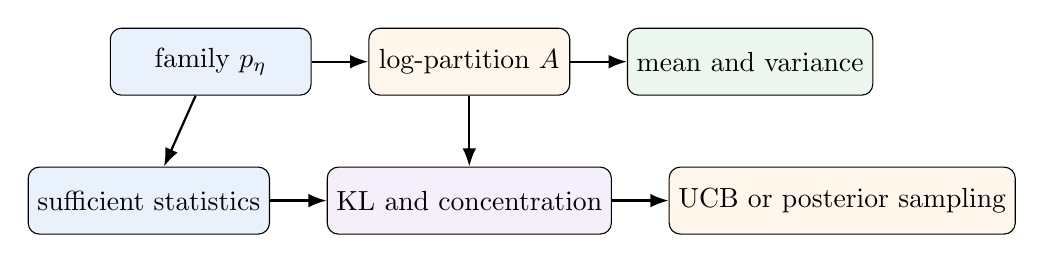
\begin{tikzpicture}[>=Latex,node distance=0.72cm]
\node[draw,rounded corners,fill=lightblue,minimum width=2.55cm,minimum height=0.85cm] (f) {family $p_\eta$};
\node[draw,rounded corners,fill=lightorange,minimum width=2.55cm,minimum height=0.85cm,right=of f] (a) {log-partition $A$};
\node[draw,rounded corners,fill=softgreen,minimum width=2.55cm,minimum height=0.85cm,right=of a] (m) {mean and variance};
\node[draw,rounded corners,fill=softpurple,minimum width=2.55cm,minimum height=0.85cm,below=0.9cm of a] (k) {KL and concentration};
\node[draw,rounded corners,fill=lightblue,minimum width=2.55cm,minimum height=0.85cm,left=of k] (s) {sufficient statistics};
\node[draw,rounded corners,fill=lightorange,minimum width=2.55cm,minimum height=0.85cm,right=of k] (d) {UCB or posterior sampling};
\draw[->,thick] (f) -- (a);
\draw[->,thick] (a) -- (m);
\draw[->,thick] (a) -- (k);
\draw[->,thick] (f) -- (s);
\draw[->,thick] (s) -- (k);
\draw[->,thick] (k) -- (d);
\end{tikzpicture}
\end{center}

This is why exponential families are a natural language for bandit theory. They do not make every model identical. They reveal which calculations are identical, which quantities remain model-specific, and where statistical evidence enters the decision rule.

\backmatter
\chapter*{Appendix A. Formula Sheet}
\addcontentsline{toc}{chapter}{Appendix A. Formula Sheet}

\begin{table}[H]
\centering
\caption*{Core formulas.}
\begin{tabular}{p{0.34\textwidth}p{0.56\textwidth}}
\toprule
Object & Formula \\
\midrule
Canonical family & $p_\eta(x)=h(x)e^{\eta T(x)-A(\eta)}$ \\
Log-partition & $A(\eta)=\log\int h(x)e^{\eta T(x)}\,\dd\nu(x)$ \\
Mean statistic & $A'(\eta)=\E_\eta[T(X)]$ \\
Variance statistic & $A''(\eta)=\Var_\eta(T(X))$ \\
Vector mean & $\nabla A(\bm\eta)=\E_{\bm\eta}[\bm T(X)]$ \\
Vector covariance & $\nabla^2A(\bm\eta)=\Cov_{\bm\eta}(\bm T(X))$ \\
Joint sufficient statistic & $S_n=\sum_{i=1}^{n}T(X_i)$ \\
MLE equation & $A'(\widehat\eta_n)=S_n/n$ \\
Conjugate prior & $\pi(\eta\mid\xi,\nu)\propto e^{\xi\eta-\nu A(\eta)}$ \\
Conjugate update & $(\xi,\nu)\mapsto(\xi+S_n,\nu+n)$ \\
Family KL & $\KL(P_\eta\Vert P_\zeta)=A(\zeta)-A(\eta)-A'(\eta)(\zeta-\eta)$ \\
Fisher information & $I(\eta)=A''(\eta)$ \\
Moment-generating function & $\E_\eta[e^{\lambda T(X)}]=e^{A(\eta+\lambda)-A(\eta)}$ \\
Chernoff exponent & $\Pbb_\eta(\overline T_n\ge x)\le e^{-n\KL(P_{\eta_x}\Vert P_\eta)}$ \\
Bandit ledger & $N_a(t),\ S_a(t)=\sum_{s\le t:A_s=a}T(X_s)$ \\
KL-UCB index & $\sup\{q:N_a d(\widehat\mu_a,q)\le\beta(t)\}$ \\
\bottomrule
\end{tabular}
\end{table}

\chapter*{Appendix B. Notation Table}
\addcontentsline{toc}{chapter}{Appendix B. Notation Table}

\begin{table}[H]
\centering
\caption*{Notation.}
\begin{tabular}{p{0.24\textwidth}p{0.66\textwidth}}
\toprule
Symbol & Meaning \\
\midrule
$X$ & one observation or reward \\
$T(X)$ & canonical statistic of one observation \\
$h(x)$ & base density or mass independent of the parameter \\
$\eta$ & natural parameter \\
$\mathcal H$ & natural-parameter space \\
$A(\eta)$ & log-partition function \\
$\mu=A'(\eta)$ & mean parameter for the statistic \\
$S_n$ & sum of sufficient statistics through $n$ observations \\
$\xi,\nu$ & conjugate-prior hyperparameters \\
$A^*$ & convex conjugate of $A$ \\
$d(\mu,q)$ & family KL divergence in mean coordinates \\
$A_t$ & arm selected at round $t$ \\
$N_a(t)$ & number of pulls of arm $a$ by time $t$ \\
$S_a(t)$ & sufficient-statistic total for arm $a$ \\
$U_a(t)$ & upper confidence index \\
\bottomrule
\end{tabular}
\end{table}

\chapter*{Appendix C. Minimal Implementation Notes}
\addcontentsline{toc}{chapter}{Appendix C. Minimal Implementation Notes}

The supplied Python script reproduces all figures and tables. A few details matter in numerical work:

\begin{enumerate}
\item Clip Bernoulli probabilities away from exactly $0$ and $1$ before taking logarithms, while preserving the limiting convention $0\log0=0$.
\item Use shape-rate consistently for Gamma distributions. NumPy and SciPy accept a scale, which is the reciprocal of the rate.
\item Invert one-sided Bernoulli or Poisson KL balls by monotone bisection. A fixed iteration count gives predictable numerical cost.
\item Initialize every arm before dividing by $N_a(t)$.
\item Treat the simulation table as an audit of the implementation, not a general ranking of algorithms.
\end{enumerate}

\chapter*{Further Reading}
\addcontentsline{toc}{chapter}{Further Reading}

Barndorff-Nielsen's monograph develops the statistical theory of exponential families in depth \cite{barndorff1978information}. Wainwright and Jordan give the modern convex-analytic view that connects exponential families, marginal polytopes, and variational inference \cite{wainwright2008graphical}. MacKay's Cambridge text is an unusually readable route through likelihood, Bayesian updating, and information geometry \cite{mackay2003information}; Bishop's treatment from Microsoft Research Cambridge is a useful machine-learning companion \cite{bishop2006pattern}. Lattimore and Szepesvari place these ideas directly inside bandit theory \cite{lattimore2020bandit}. For Thompson sampling in one-dimensional exponential families, see Korda, Kaufmann, and Munos \cite{korda2013thompson} and the finite-time development of Jin and collaborators \cite{jin2022expts}.


\chapter*{Appendix D. Full Experiment Script}
\addcontentsline{toc}{chapter}{Appendix D. Full Experiment Script}

\lstinputlisting[style=blogcode,language=Python,basicstyle=\ttfamily\scriptsize]{assets/exponential-families/exponential-families-simulation.py}

\nocite{barndorff1978information,brown1986fundamentals,wainwright2008graphical,mackay2003information,bishop2006pattern,ghahramani2015probabilistic,banerjee2005bregman,lattimore2020bandit,lai1985,garivier2011klucb,korda2013thompson,jin2022expts}
\printbibliography

\end{document}
